\documentclass[dvipdfmx, 11pt, aspectratio=169]{beamer}   % dvipdfmx で非 ASCII 画像も安全
\usetheme{metropolis}
\usecolortheme{metropolis}
\usepackage{booktabs}
\usepackage{ulem}
\usepackage{tabularx}
\newcolumntype{L}{>{\raggedright\arraybackslash}X} % 左寄せの X 列
\usepackage{graphicx}
\usepackage{amsmath}
\usepackage{bm}
\usepackage{listings}
\usepackage{xcolor}
% コードのハイライト設定
\definecolor{codegreen}{rgb}{0,0.6,0}
\definecolor{codegray}{rgb}{0.5,0.5,0.5}
\definecolor{codepurple}{rgb}{0.58,0,0.82}
\definecolor{backcolour}{rgb}{0.95,0.95,0.92}

\definecolor{strongpink}{RGB}{233,30,99} % 鮮やかなピンク(参考: Material Design Pink 500)
\lstdefinestyle{mystyle}{
    backgroundcolor=\color{backcolour},   
    commentstyle=\color{codegreen},
    keywordstyle=[1]\color{blue},
    keywordstyle=[2]\color{teal},
    keywordstyle=[3]\color{strongpink},
    numberstyle=\tiny\color{codegray},
    stringstyle=\color{codepurple},
    basicstyle=\ttfamily\scriptsize,
    breakatwhitespace=false,         
    breaklines=true,                 
    captionpos=b,                    
    keepspaces=true,                 
    numbers=left,                    
    numbersep=5pt,                  
    showspaces=false,                
    showstringspaces=false,
    framexleftmargin=2em,
    showtabs=false,                  
    tabsize=2
}

\lstdefinelanguage{CUDA}{
  language=[ANSI]C++,                % C++ を継承
  morekeywords={
    __global__,__device__,__shared__,__constant__,__managed__,cudaError_t,
    __syncthreads,atomicAdd,atomicSub,atomicExch,dim3,blockIdx,threadIdx
  }
}

\lstdefinestyle{makefilestyle}{
  language        = make,        % listings 標準の make 言語
  basicstyle      = \ttfamily\footnotesize,
  keywordstyle    = \color{blue}\bfseries,
  commentstyle    = \color{codegreen},
  stringstyle     = \color{codepurple},
  numbers         = left,        % 行番号
  numberstyle     = \scriptsize\color{codegray},
  stepnumber      = 1,
  numbersep       = 6pt,
  tabsize         = 4,           % TAB=4 スペース
  showstringspaces= false,
  showtabs        = false,
  breaklines      = true,
  morekeywords    = {CC,CXX,LD,AR,CFLAGS,CXXFLAGS,LDFLAGS,RM,\%.o,all,clean}, % 独自キーワード
  xleftmargin     = 2em,         % コードブロック全体を右へ
  frame           = single,      % 枠線
  backgroundcolor = \color{backcolour}
}

\lstdefinelanguage{CSL}{
  language=[ANSI]C++,            % C++を継承
  morekeywords=[1]{
    bool, u8, u16, u32, u64, i8, i16, i32, i64, f16, f32, bf16, 
    task, function, extern, dsd, register, fabric, volatile, 
    struct, const, static, inline, uniform, comptime_struct
    blockid, peid, colorid, color, queue, numpes, numtids,
    layout, runner
  },
  morekeywords=[2]{
    @send_to_color, @send_to_host, @activate, @block, @unblock,
    @recv_from_color, @wait_until_empty, @clear,
    @fadds, @fsubs, @fmuls, @fmacs, @reduce_add, @reduce_max,
    @fmovs, @copy, @fexps, @flogs, @frelus, @fsum, @fmax,
    @fetch, @push, @pop, @peek, @capacity, @fill,
    @get_dsd, @get_dsr, @load_to_dsr, @get_ut_id,
    @set_rectangle, @set_tile_code, @import_module, @export_name
  },
  morekeywords=[3]{
    memcpy_d2h, load, run, launch, base_address, 
    offset, stride, extent, tensor_access, width, height,
    async, activate, element_type
  }
  sensitive=true,               % 大文字小文字を区別
  morecomment=[l]{//},          % 行コメント
  morecomment=[s]{/*}{*/},      % ブロックコメント
  morestring=[b]",              % 文字列
  morestring=[b]'               % 文字
}

\lstset{language=CSL}  % デフォルト言語としてCSLを設定
\usepackage{hyperref}
% URLの#記号をエスケープするための設定
\makeatletter
\g@addto@macro\UrlSpecials{\do\#{\char35 }}
\makeatother
\newcommand{\ulhref}[2]{\href{#1}{\textcolor{cyan}{\uline{#2}}}}
\lstset{style=mystyle}
\title{Cerebras System: remarkable hardware accelarator and its programming model}
\author{Yuri Takigawa}
\institute{The university of Tokyo, EEIC, Taura Lab}
\date{\today}

%%%%%%%%%%%%%%%%%%%%%%%%%%%%%%%%%%%%%%%%
\begin{document}
%%%%%%%%%%%%%%%%%%%%%%%%%%%%%%
% タイトルスライド
\begin{frame}
  \titlepage       
\end{frame}
% 目次スライド
\begin{frame}
  \frametitle{Contents}
  \tableofcontents
\end{frame}
%%%%%%%%%%%%%%%%%%%%%%%%%%%%%%%
\section{Installation and Setup}
%%%%%
\begin{frame}
    \frametitle{Contents}
    \tableofcontents[currentsection]
\end{frame}
%%%%%
\begin{frame}{How to get an access to SDK}
Fill the form on this \ulhref{https://www.cerebras.ai/developers/sdk-request}{link}.
\begin{itemize}
    \item Human operators reply, thus it takes more than half a day.
    \item The reply includes \textbf{Dropbox link} to the \textbf{SDK files}.
\end{itemize}
Most of the things about \textbf{installation and setup} are \ulhref{https://sdk.cerebras.net/installation-guide}{here}.
\begin{itemize}
    \item The most important thing is that \uwave{this SDK is for \textbf{amd64} architecture}.
\end{itemize}
\end{frame}
%%%%%
\begin{frame}[fragile]{Overview of installation and setups}
Some of the (critical) things below are \textbf{NOT} explicitly written in the \ulhref{https://sdk.cerebras.net/installation-guide}{guide}.
\begin{enumerate}
    \item \textbf{Azure VM} is highly recommended as an environment (\textbf{Miyabi} is not available here...)
    \begin{itemize}
        \item Recommended instance type is \textbf{Standard B4ms} (4vcpu, 16GiB memory) with 64GiB disk.
    \end{itemize}
    \item When you connect via \textbf{ssh}, \lstinline|ssh -i ~/.ssh/YOUR_PRIVATE_KEY -Y -L 8000:localhost:8000 YOUR_USERNAME@PUBLICIP|
    \begin{itemize}
        \item transfer \textbf{port 8000} to remote \textbf{port 8000}
        \item \lstinline|YOUR_USERNAME| is \textbf{NOT} a resource name.
        \item \lstinline|YOUR_PUBLICIP| can be seen on the resource via \ulhref{https://portal.azure.com/?feature.msaljs=true\#home}{azure home}
        \item You can also refer past \ulhref{https://gitlab.eidos.ic.i.u-tokyo.ac.jp/eidos/labdocs/-/tree/master/spring-training/2025/05-environment-setup-azure?ref_type=heads}{spring-training} by gotonao
    \end{itemize}
\end{enumerate}
\end{frame}
%%%%%
\begin{frame}{Overview of installation and setups}
\begin{enumerate}\setcounter{enumi}{2}
    \item You can follow the \ulhref{https://sdk.cerebras.net/installation-guide}{guide} at installation/setup, but some filenames are changed.
    \item Finally, you can try remote GUI debug (step7 of the guide).
    \begin{itemize}
        \item \lstinline|sdk_debug_shell visualize| after running the test, open \lstinline|http://localhost:8000/sdk-gui| at your local browser (eg. chrome)
        \item Sometimes, version conflict occurs and show a kind of bugs.
    \end{itemize}
\end{enumerate}
%%
\begin{figure}
    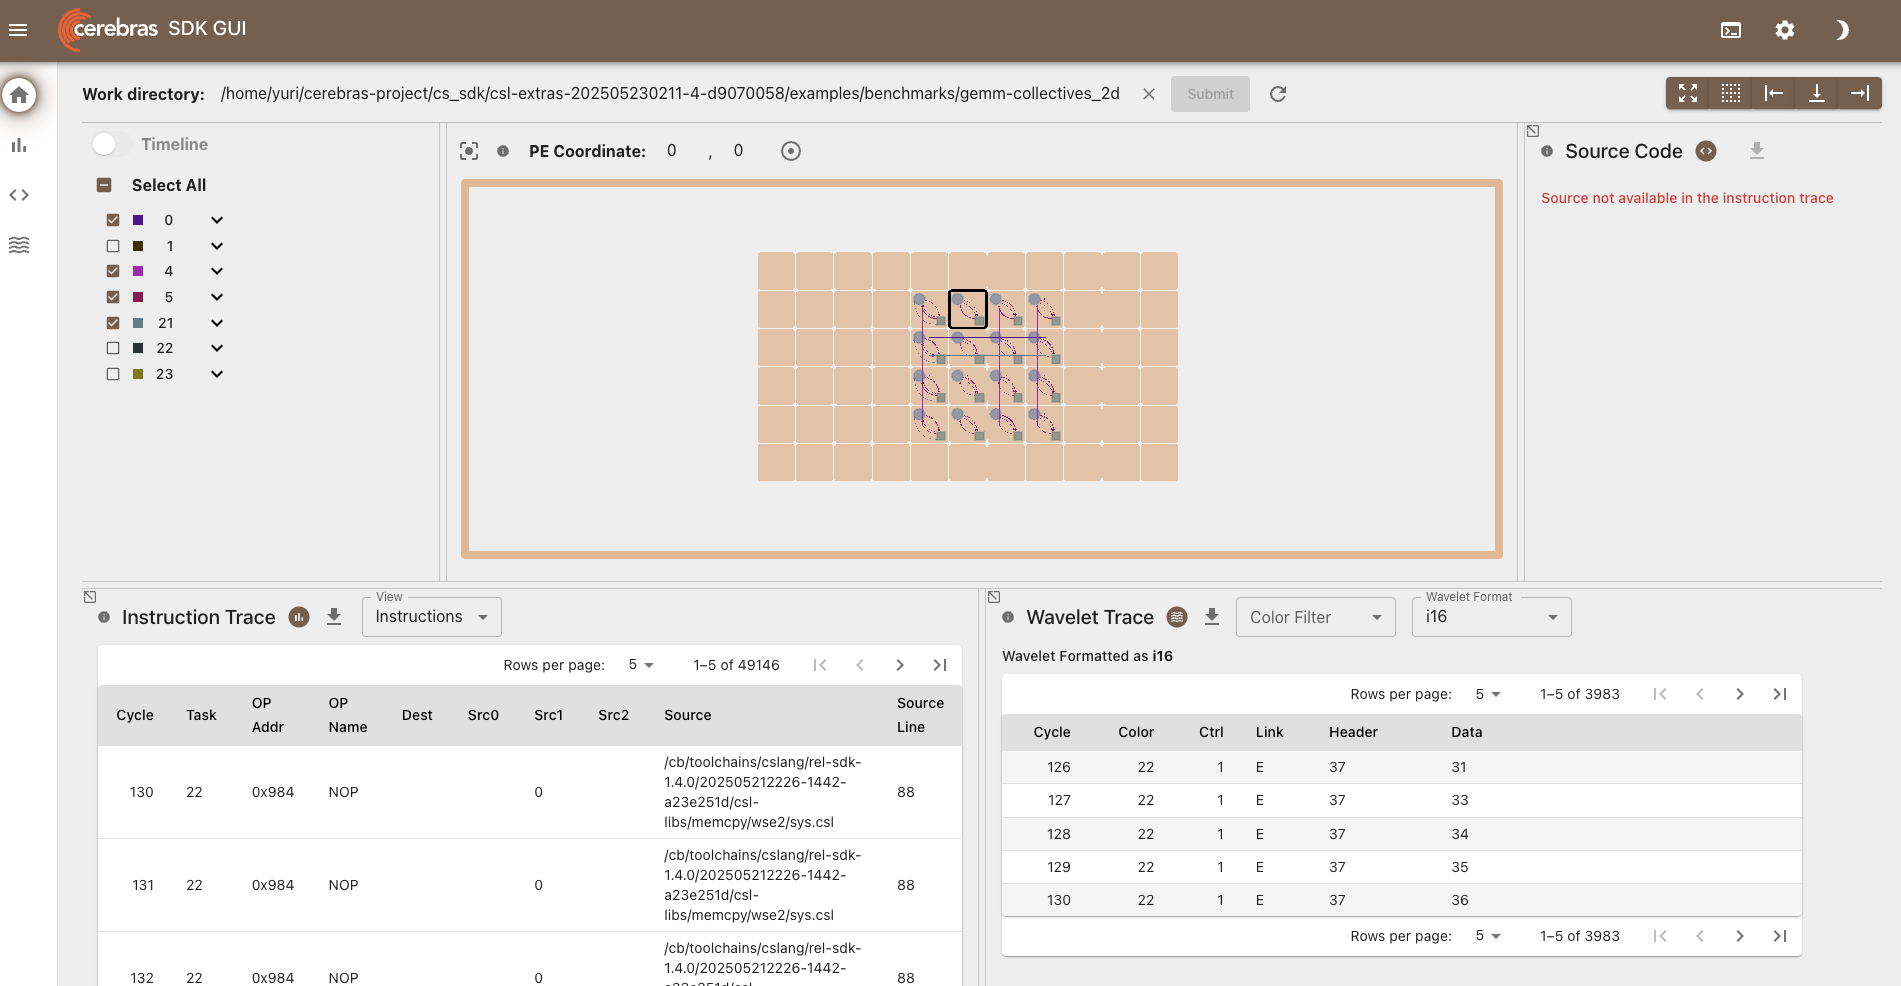
\includegraphics[scale=0.12]{img/sdk-gui.png}
\end{figure}
\end{frame}
%%%%%%%%%%%%%%%%%%%%%%%%%%%%%%%
\section{A Conceptual View: Hardware organization}
% table of contents
\begin{frame}
    \frametitle{Contents}
    \tableofcontents[currentsection, hideothersubsections]
\end{frame}
%%%%%%%%%%%%%%%%
\subsection{PE (Processing Elements)}
%%%%%
\begin{frame}{Wafer Scale Engine}
\textbf{Cerebras} refers its hardware accelarator as a \textbf{WSE (Wafer Scale Engine)}.
%%
\begin{itemize}
    \item WSE consists of hundreds (dies) of thousands (数千万個) of independent \textbf{PE} (processing element)s ($\sim$ cores).\footnote{uses TSMC $5$nm processed node}
    \item The PEs are interconnected by communication links, and they form a \textcolor{blue}{two-dimensional rectangular mesh} on one single silicon wafer.
\end{itemize}
%%
\begin{figure}
    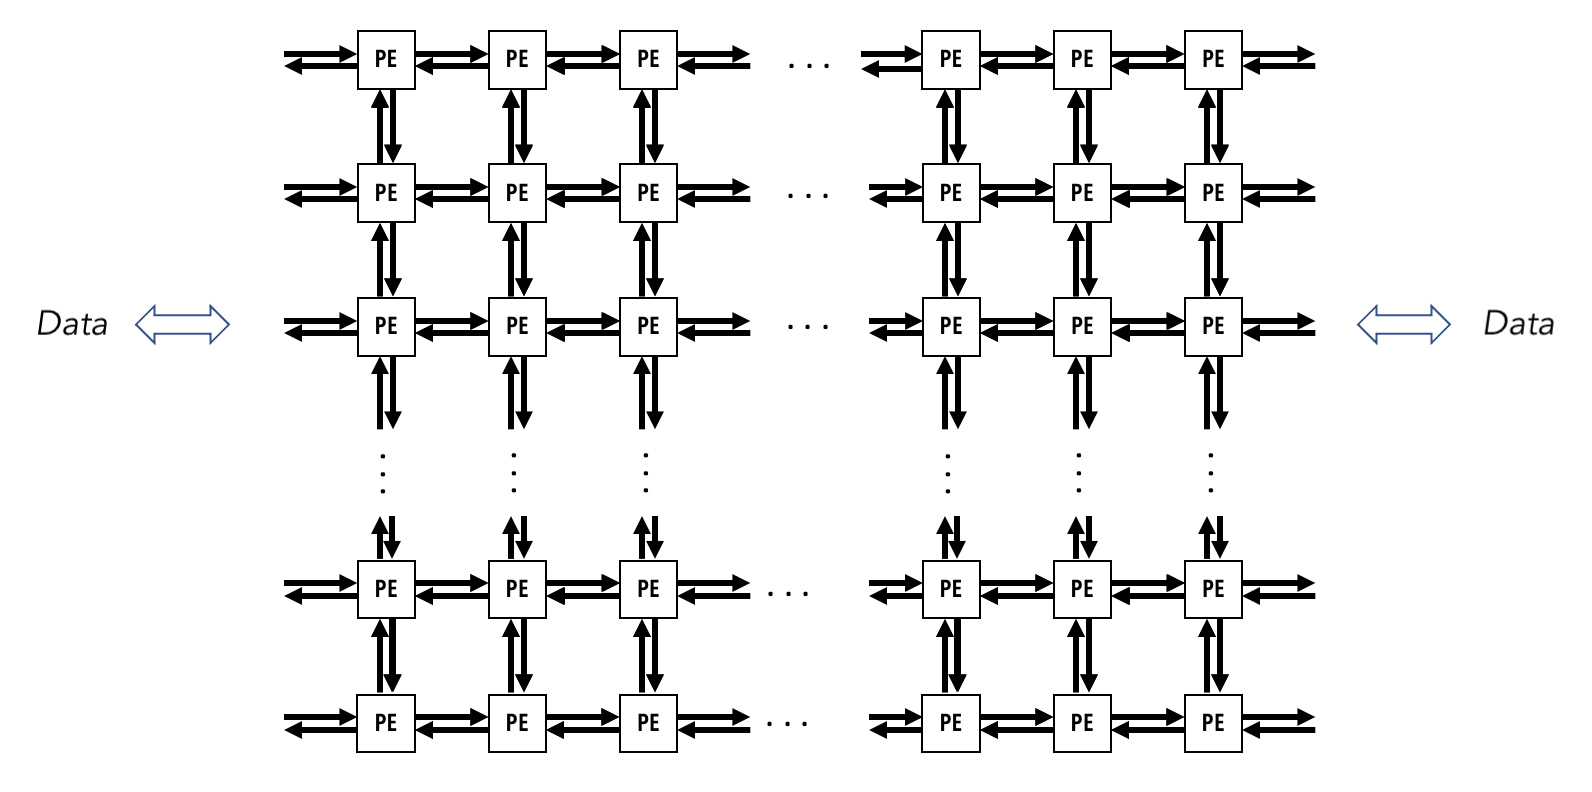
\includegraphics[scale=0.14]{img/cs-mesh.png}
\end{figure}
\end{frame}
%%%%%
\begin{frame}{Characteristics of a PE: memory}
\begin{columns}
\column{0.65\textwidth}
\begin{itemize}
    \item Each PE has its own \textbf{physically-local SRAM} (called \textbf{local PE memory}) \footnote{200x normalized memory BW vs. GPU} with single-cycle access.
    \begin{itemize}
        \item is $48$kB total, consists of $8$ banks, and has full datapath bandwidth: 2 64(128)bit read + 1 64(128)bit write per cycle
        \item each bank has $6$kB, and $32$bit wide, has single port
    \end{itemize}
    \item All the code and data related to the execution on the PE are stored \textcolor{blue}{within} this memory.
    \item This physically-local memory is \textbf{logically local} as well (i.e., No other PE are directly accessible to this memory)
\end{itemize}
%%
\column{0.35\columnwidth}
\vspace{-\baselineskip}
\begin{figure}
    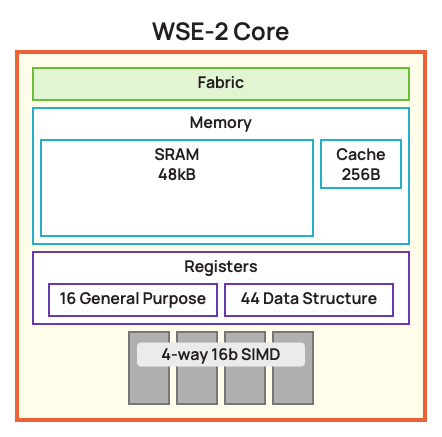
\includegraphics[scale=0.22]{img/wse2Core.png}\\
    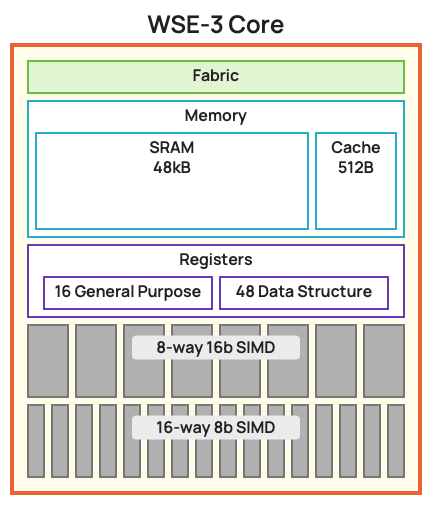
\includegraphics[scale=0.22]{img/wse3Core.png}
\end{figure}
\end{columns}
\end{frame}
%%%%%
\begin{frame}{Characteristics of a PE: processor}
\begin{columns}
\column{0.65\textwidth}
\begin{itemize}
    \item Each PE has a \textbf{processor} called \textbf{CE (Compute Engine)}.
    \begin{itemize}
        \item $16$ general purpose registers, $48$ data structure registers
        \item Compact $6$-stage pipeline
        \item Flexible \textcolor{blue}{general ops} (e.g., arithmetic, logical, load/store, compare, branch) for control processing
    \end{itemize}
    \item CE has \textbf{SIMD} computing unit
    \begin{itemize}
        \item In the WSE2, \textbf{$4$-way 16 bit SIMD}\footnote{which means execute single instruction with 4 different data simultaneously}, each way has ALU for FADD, FMUL, FMAC\footnote{Fused Multiply-Add} etc.,
        \item In the WSE3, \textbf{$8$-way 16 bit SIMD} and \textbf{$16$-way 8 bit SIMD}
    \end{itemize}
\end{itemize}
%%
\column{0.35\columnwidth}
\vspace{-\baselineskip}
\begin{figure}
    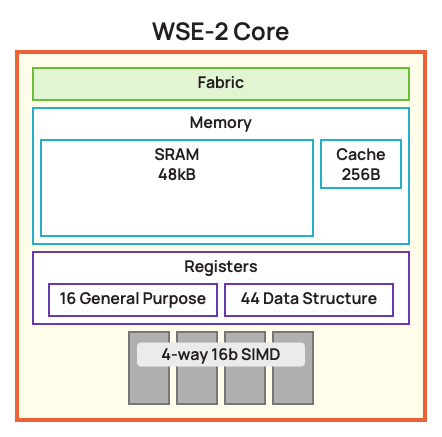
\includegraphics[scale=0.22]{img/wse2Core.png}\\
    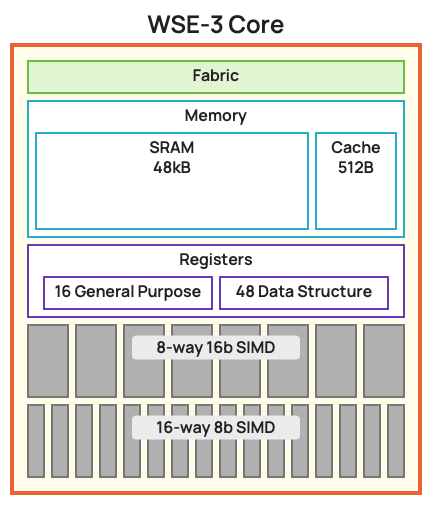
\includegraphics[scale=0.22]{img/wse3Core.png}
\end{figure}
\end{columns}
\end{frame}
%%%%%
\begin{frame}{Characteristics of a PE: processor}
\begin{itemize}
    \item Each PE has its own independent PC (program counter).
    \begin{itemize}
        \item Thus, each PE can execute codes \textcolor{blue}{asynchronously} by default.
    \end{itemize}
\end{itemize}
%%
\begin{figure}
    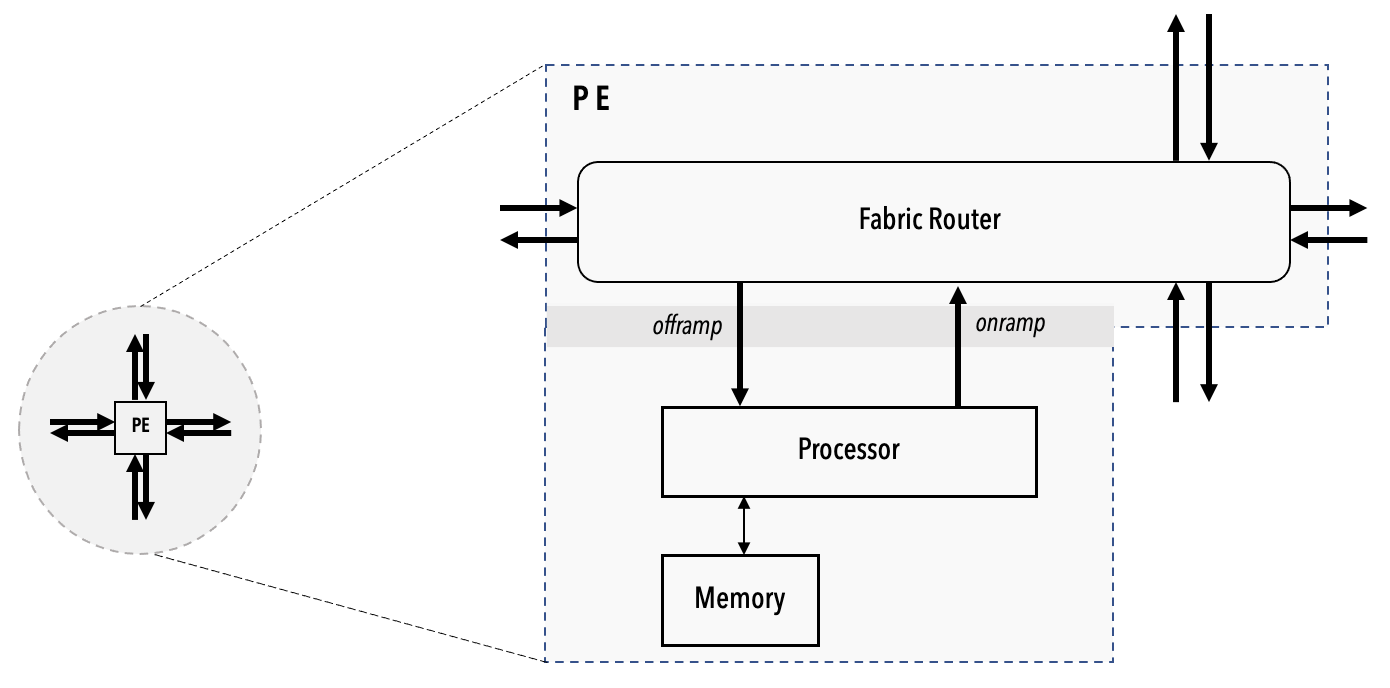
\includegraphics[scale=0.15]{img/pe-symbolic.png}
\end{figure}
\end{frame}
%%%%%
\begin{frame}{Characteristics of a PE: router}
\begin{itemize}
    \item Each PE has the hardware unit for communication (send, receive) called \textbf{Router}.
    \item A \textbf{Router} is directly connected to its own \textbf{CE} via \textcolor{blue}{bidirectional} link called \textbf{RAMP (Router ALU Messaging Path)}.\footnote{You may have heard this word as インターチェンジ of highway} 
    \item A \textbf{Router} is directly connected to the routers of the four nearest neighboring PEs (north, south, east, west)
    \begin{itemize}
        \item Thus, a router has $4$ ports
    \end{itemize}
    \item A \textbf{Router} has $8$ \textbf{input queue}s and \textbf{output queue}s inside the PE.
    \begin{itemize}
        \item An \textbf{input queue} is a \textcolor{blue}{hardware buffer} where data is temporarily stored before the entering the CE. (I will explain what this means later)
    \end{itemize}
\end{itemize}
% %%
% \begin{figure}
%     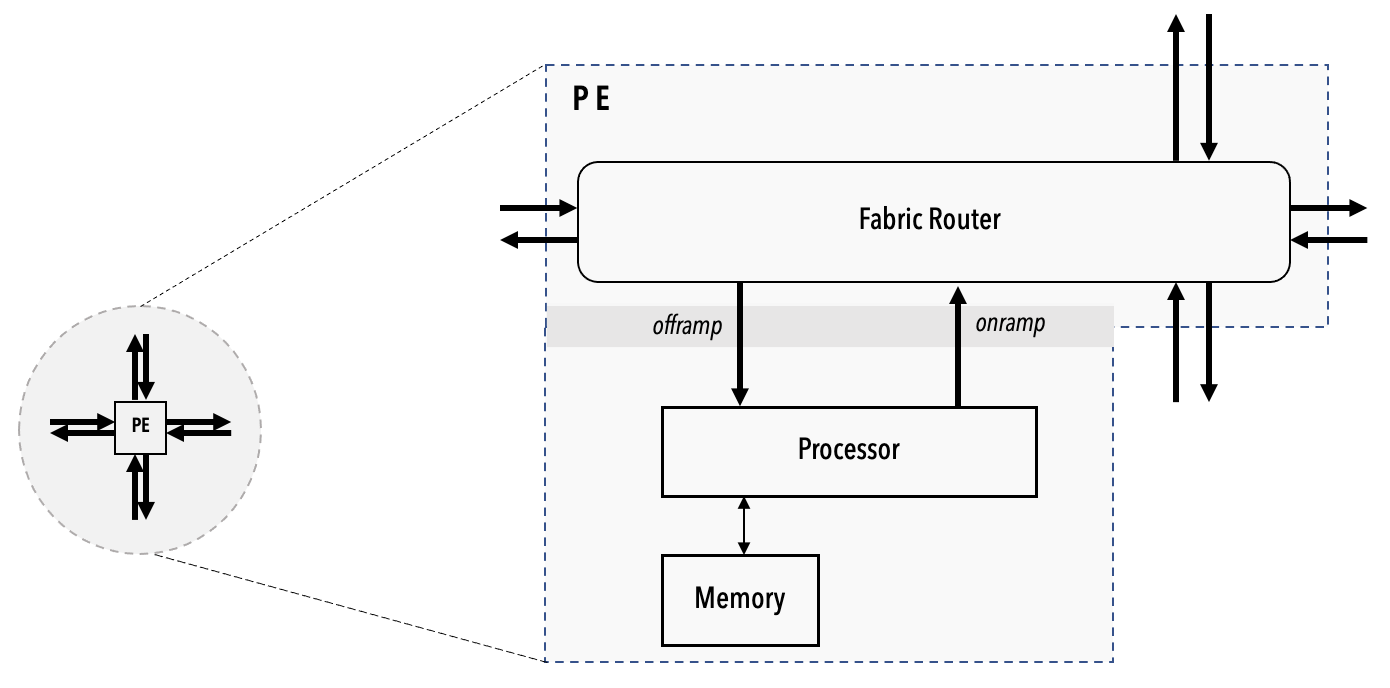
\includegraphics[scale=0.15]{img/pe-symbolic.png}
% \end{figure}
% %%
\end{frame}
%%%%%%%%%%%%%%%%%%%%%
\section{A Conceptual View: Programming model}
% table of contents
\begin{frame}
    \frametitle{Contents}
    \tableofcontents[currentsection, hideothersubsections]
\end{frame}
%%%%%%%%%%%%%%%%%
\subsection{Programming Language}
%%%%%
\begin{frame}[fragile]{Programming Language: CSL}
\begin{itemize}
    \item To develop code for the WSE, write \textit{device code} in the \textbf{CSL (Cerebras Software Language)}, and \textit{host code} in \textit{Python}.
    \begin{itemize}
        \item The host code is responsible for \textbf{copying data to and from the device}
        \item \textbf{CSL} gives programmers full control of the \textbf{WSE}.
    \end{itemize}
    \item Then, compile the \textit{device code} with \lstinline|cslc|, and run your program on either \textbf{Cerebras fabric simulator} (or the actual network-attached device).
    \begin{itemize}
        \item The usage is \ulhref{https://sdk.cerebras.net/csl/csl-compiler}{here}.
    \end{itemize}
\end{itemize}
\end{frame}
%%%%%
\begin{frame}{Programs and Tasks}
%%
A \textbf{CSL program} consists of one or more \textit{subprograms}.

Subprogram has two \textbf{types} (declaration).
\begin{itemize}
    \item \textbf{function}: callable
    \item \textbf{task}: a procedure that cannot be called from other code
    \begin{itemize}
        \item something like \textcolor{blue}{atomic} (i.e., unsplittable) code block managed by hardware
        \item tasks are managed at \textit{the specialized hardware unit} of \textbf{CE} similar to rich \textit{NPC generator}
        \item A task can be \textcolor{blue}{activated} (i.e., ready for running) by some \textit{hardware trigger} (imagine a flip of a flag bit)
        \item tasks are started by PE hardware (specifically \textit{NPC generator} of \textbf{CE})
        \item Only \textbf{one} task can be executed at a time on the CE
        \item Once a task is started by hardware, \uwave{it runs until it complete}. Then, the \textit{NPC generator} chooses a new task to run.
    \end{itemize}
\end{itemize}
%%
\end{frame}
%%%%%%%%%%%%%%%%%%%%%%%%%%
\subsection{Communication}
%%%%%
\begin{frame}{The unit of communication between PEs: wavelet}
$32$-bit messages ($\sim$ packets), called \textbf{wavelet}s, can be sent to or received by neighboring PEs \textcolor{blue}{in a single clock cycle}.
\begin{itemize}
    \item Arrivals of wavelets trigger something inside the PE
    \begin{itemize}
        \item \textbf{Task Activation}
        \item \textbf{Stored in a \textcolor{blue}{data struct} managed with a fabric DSD}
    \end{itemize}
    \item transfering data of massive size (like array, tensor) is \textcolor{blue}{splitted into multiple wavelets}, 
        and data of wavelets that arrive at the destination PE first is \textcolor{blue}{buffered} in the \textbf{input queue} until all wavelets arrive.
\end{itemize}
\begin{figure}
    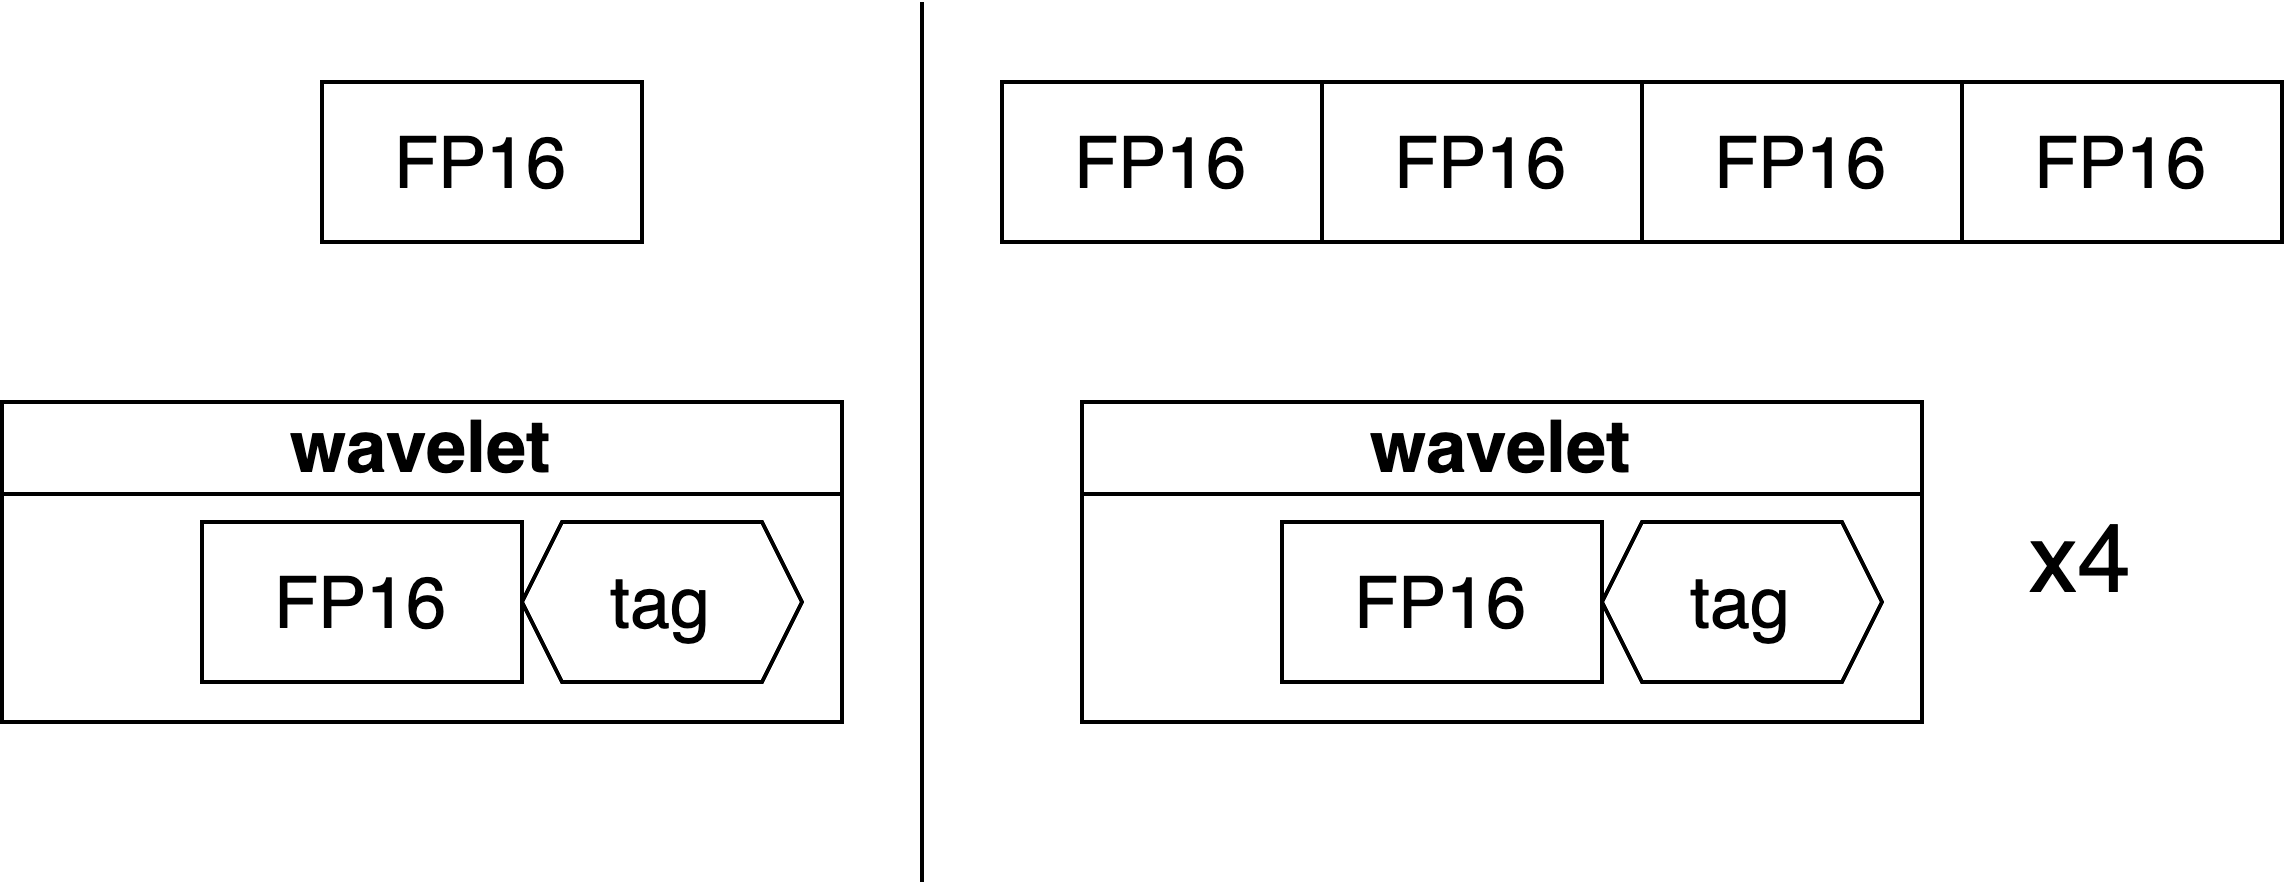
\includegraphics[scale=0.08]{img/wavelet.png}
\end{figure}
\end{frame}
%%%%%
\begin{frame}{Virtual Communication Channel: Color}
The virtual communication path (channel) through which \textbf{wavelet}s (packets) travel is called \textbf{color}.
\begin{itemize}
    \item There exists $24$ virtual channels used by hardware.
    \item All colors transfer data on a single physical channel.
    \begin{itemize}
        \item If multiple colors have wavelets to send via physical path from PE \texttt{X} to PE \texttt{Y}, those \textcolor{red}{colors (not wavelets)} are scheduled by \textbf{hardware arbiter} on router.
        \item \textbf{IMPORTANT:} The congestion of one color does \textbf{NOT} block traffic of another color; \textcolor{blue}{Fairness} between colors (not wavelets)
        \item For example, RR algorighm could be used as a policy.
    \end{itemize}
    \item Each \textbf{wavelet} has a $5$-bit \textcolor{blue}{tag} that encodes its \textbf{color}
\end{itemize}
\end{frame}
%%%%%%%%%%%%%%%%%
\subsection{Code Execution Unit: Task}
%%%%%
\begin{frame}
    \frametitle{Contents}
    \tableofcontents[currentsubsection, hideothersubsections]
\end{frame}
%%%%%
\begin{frame}{Task IDs and Types of Tasks}
Each task can be associated with \textbf{task ID} from $0$ to $63$.
\begin{itemize}
    \item \textbf{Data Task}: the arrival of wavelet triggers its activation, its \textbf{ID} is associated with a \textbf{input queue} on the \textbf{router}\footnote{In the WSE2, task ID is directly associated with the \textbf{color} with implicit linkage between \textbf{input queue} and task ID}
    \item \textbf{Local Task}: the \lstinline|@activate(task_id)| in some other codes within the same PE triggers its activation, 
    \item \textbf{Control Task}: controls other tasks on the same PE as follows, its \textbf{ID} can take any values from $0$ to $63$.
    \begin{itemize}
        \item unblock other \textbf{data task}
        \item conditional launch of \textbf{local task}
    \end{itemize}
\end{itemize}
\end{frame}
%%%%%
\begin{frame}[fragile]{The conditions to be ready for execution}
There are two \textcolor{blue}{conditions} for tasks be scheduled by \textbf{task picker} (hardware selector)
\begin{itemize}
    \item \textbf{Activated}
    \begin{itemize}
        \item every task is \textbf{inactive} by default
        \item programmers can activate the task within the same PE, with \lstinline|@activate(task_id)|.
        \item programmers can activate the task in another PE, with \lstinline|@send_to_color(output_queue_id)|.
    \end{itemize}
    \item \textbf{Unblocked} 
    \begin{itemize}
        \item every task is \textbf{unblocked} by default
        \item but, programmers can block the ID of a task at compile time, with \lstinline|@block(task_id)|.
    \end{itemize}
\end{itemize}
\end{frame}
%%%%%
\begin{frame}{Psuedo Image of hardware that manages Data Task}
\begin{figure}
    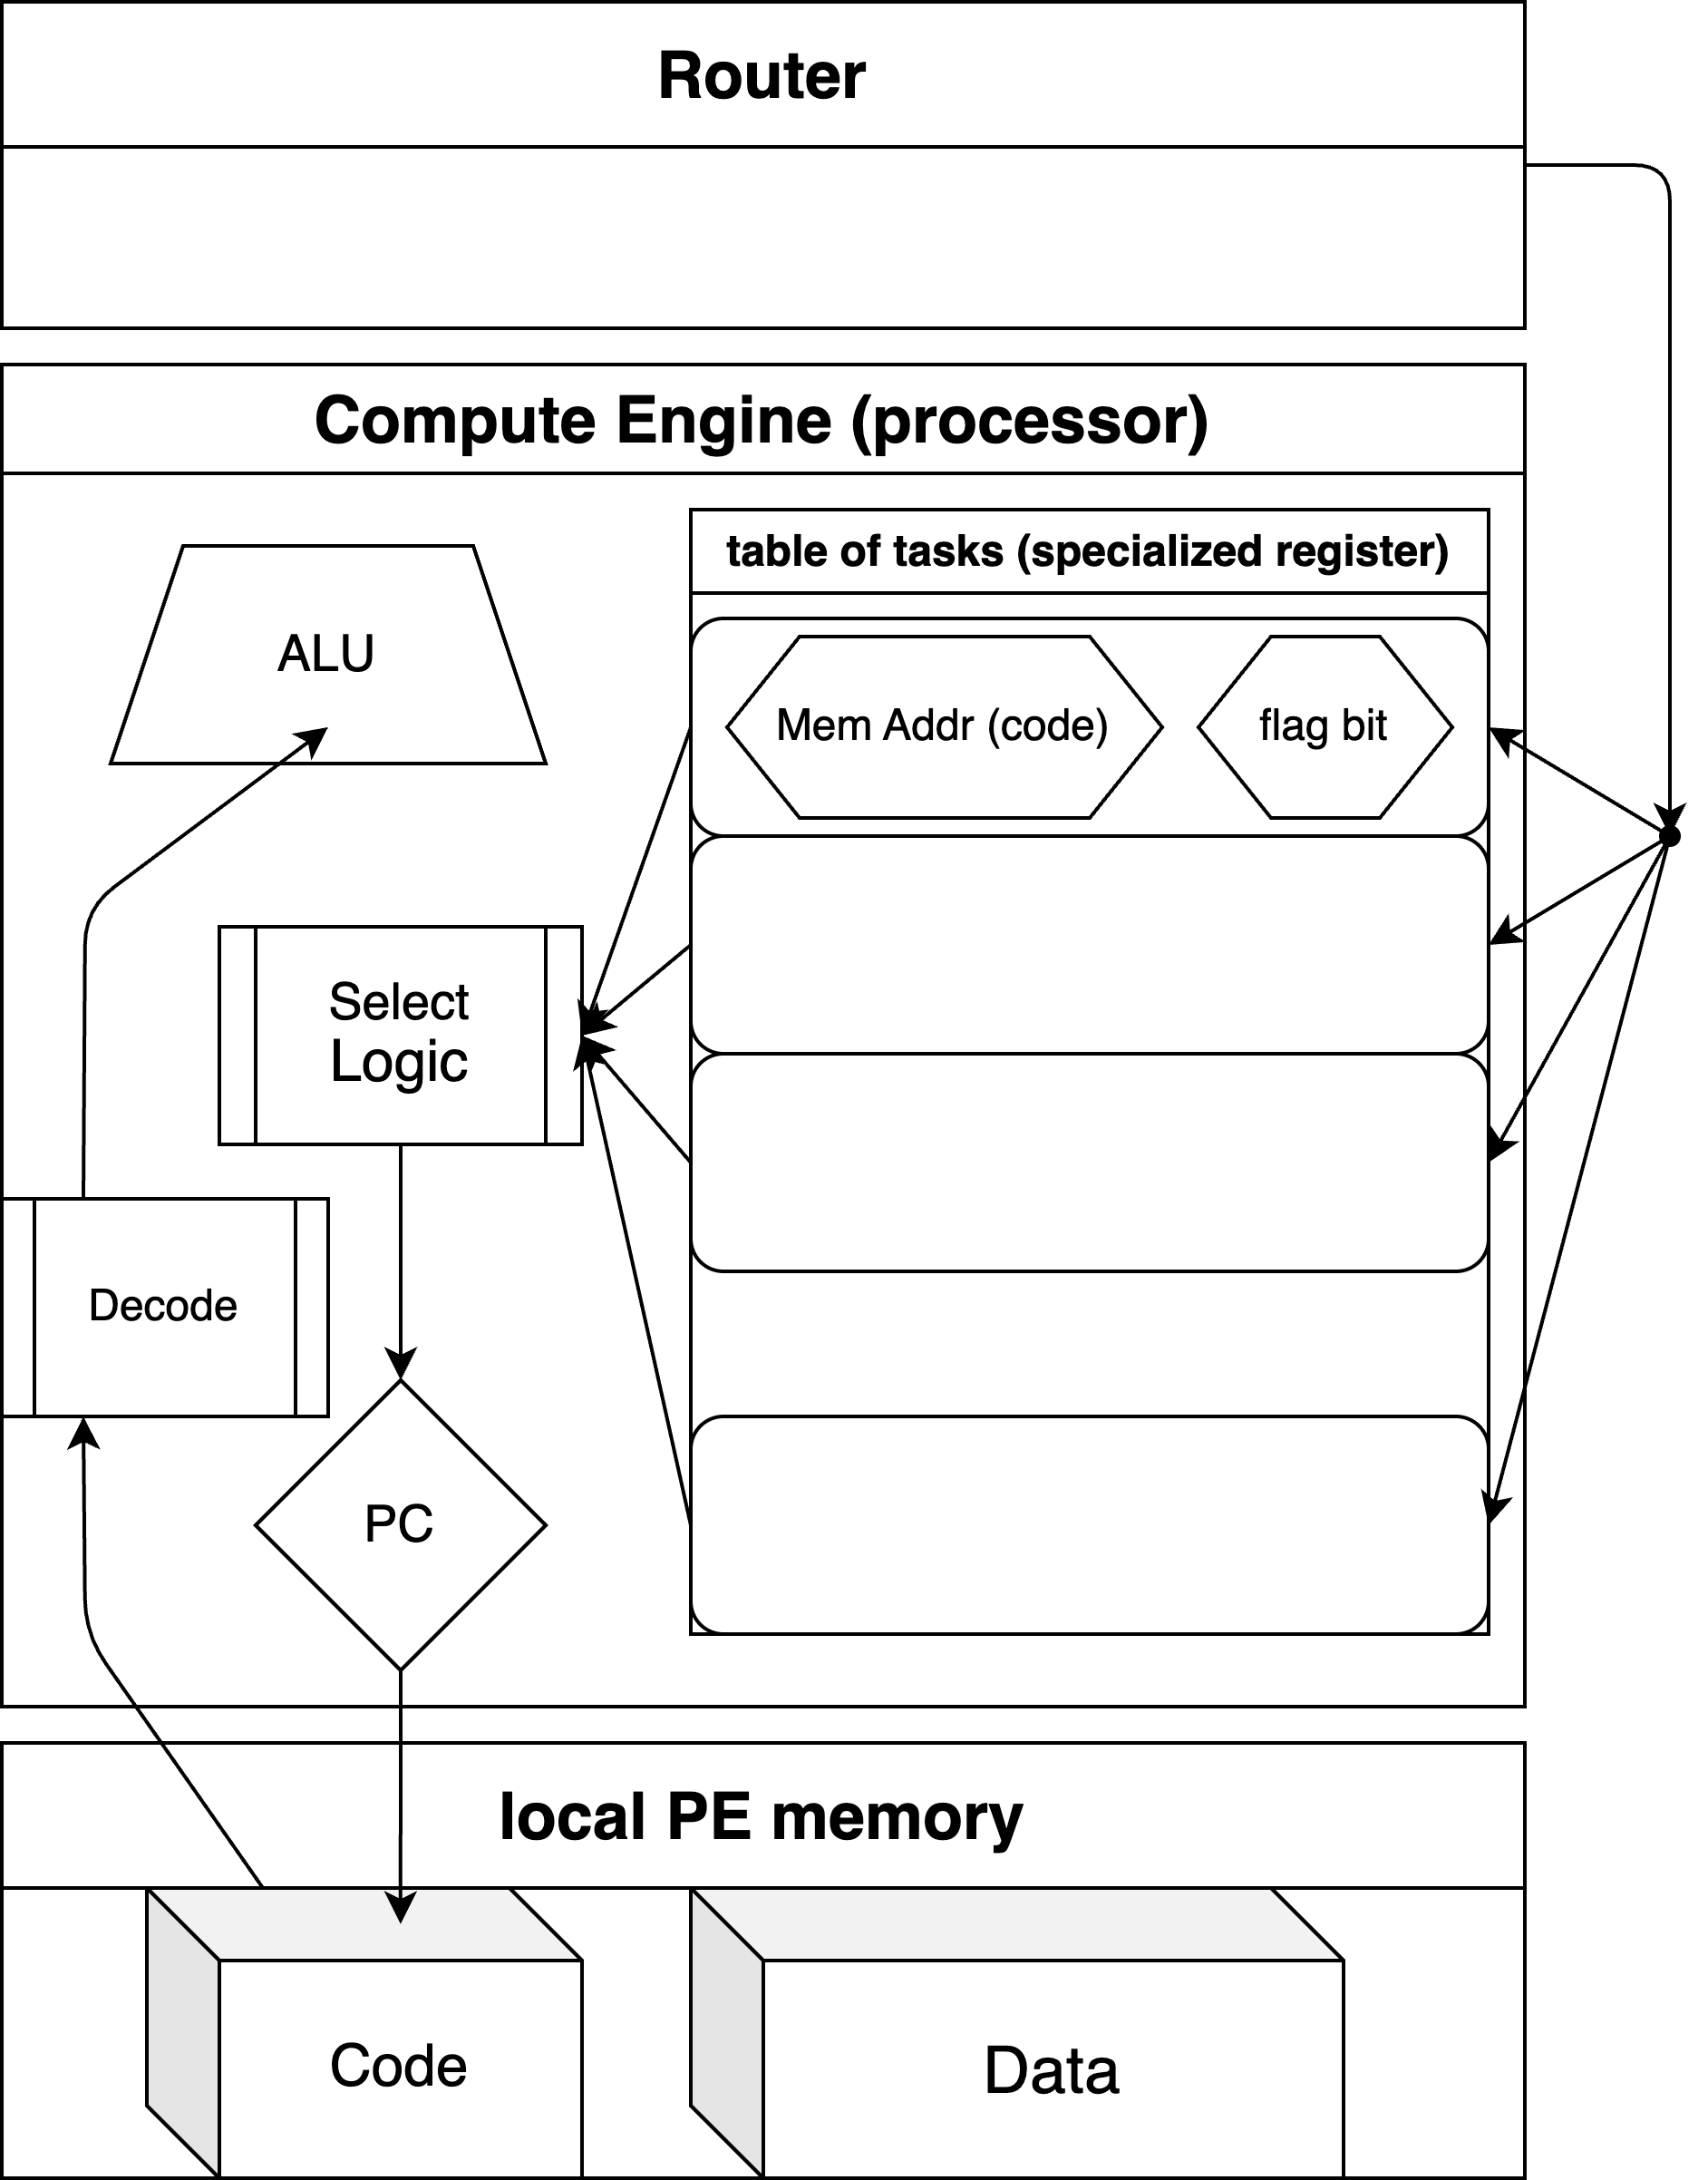
\includegraphics[scale=0.08]{img/npcGen.png}
\end{figure}
\end{frame}
%%%%%
\begin{frame}{Communication via router: Task activation}
Three
\end{frame}
%%%%%
\begin{frame}{Code Template: link computation and communication using Task}
\begin{itemize}
\item 
\end{itemize}
\end{frame}
%%%%%%%%%%%%%%%%%%%%%%%%%%
\subsection{Another use of wavelet arrival : Data Struct}
%%%%%
\begin{frame}
    \frametitle{Contents}
    \tableofcontents[currentsubsection]
\end{frame}
%%%%%
\begin{frame}[fragile]{Preliminaries: the hardware instruction of Tensor}
\begin{columns}
\column{0.54\textwidth}

CSL supports several \textbf{tensor ops}
\begin{itemize}
    \item Every tensor op has its options
    \begin{itemize}
        \item asynchronous execution means, release software serialization 
        \item i.e., start execution even before the previous op is completed, considering whether or not hazard (data, structural) exist
    \end{itemize}
\end{itemize}
\vspace{-0.5\baselineskip}
\begin{lstlisting}[language=CSL, basicstyle=\ttfamily\tiny]
.{
  .async = true,            // asynchronous execution flag
  .activate = task_id,      // task id of the task activated when this op completes
  .element_type = f32,      // type
  // other options specific to each op
}
\end{lstlisting}
\vspace{-0.5\baselineskip}
\begin{itemize}
    \item The format of these ops are (\ulhref{https://sdk.cerebras.net/csl/language/builtins\#language-builtins-for-dsd-operations}{here}):
\end{itemize}
%%
\column{0.01\textwidth}
\centering\vrule width 0.4pt
%%
\column{0.45\textwidth}
\begin{lstlisting}[language=CSL, basicstyle=\ttfamily\tiny]
// ARITHMETIC
// dst = src1 * src2 + acc
@fmacs(dst, acc, src1, src2 [, options])
// dst = src1 {+, -, *, /} src2
@fadds(dst, src1, src2 [, options])
@fsubs(dst, src1, src2 [, options])
@fmuls(dst, src1, src2 [, options])
@fdivs(dst, src1, src2 [, options])

// COPY
// dst = src
@fmovs(dst, src [, options])
// dst = src(size)
@copy(dst, src, size_in_bytes)

// ELEMENT-WISE OPS
@fexps(dst, src [, options])    // exp
@flogs(dst, src [, options])    // ln
@frelus(dst, src [, options])   // ReLU

// REDUCTION OPS
@fsum(dst, src [, options]) // sum of items
@fmax(dst, src [, options]) // dst is scaler
\end{lstlisting}
\end{columns}
\end{frame}
%%%%
\begin{frame}[fragile]{DSD: Abstraction of data consists of multiple values like tensor}
\textbf{Data Structure Descriptors (DSDs)}      [More details are available \ulhref{https://sdk.cerebras.net/csl/language/dsds\#data-structure-descriptors}{here}.]
\begin{itemize}
    \item are a \textcolor{blue}{compact representation} of 
    \begin{itemize}
        \item a chunk of memory (or)
        \item a sequence of incoming or outgoing wavelets
    \end{itemize}
    \item enable various \textcolor{blue}{repeated operations} to be expressed using just \textcolor{blue}{one hardware instruction}
    \item is an software object which consists of
    \begin{itemize}
        \item \lstinline|dst_type|: one of \lstinline|mem1d_dsd|, \lstinline|mem4d_dsd|, \lstinline|fabin_dsd|, or \lstinline|fabout_dsd|
        \item properties: different \lstinline|dst_type| has different properties
    \end{itemize}
\end{itemize}
\begin{columns}
\column{0.48\textwidth}
\begin{lstlisting}[language=CSL, basicstyle=\ttfamily\tiny]
// A 'mem1d_dsd' created through explicitly specifying properties
const dsd1 = @get_dsd(mem1d_dsd, .{
        .base_address = access_of_A.base_address,
        .offset = access_of_A.offset,
        .stride = access_of_A.stride,
        .extent = access_of_A.extent});
\end{lstlisting}
\column{0.48\textwidth}
\begin{lstlisting}[language=CSL, basicstyle=\ttfamily\tiny]
// 'access_of_A' is exactly equivalent to: 
// .{.base_address = &A, .offset = 42, .stride = .{2}, .extent = .{10}}
const access_of_A: comptime_struct 
                    = |i|{10} -> A[2*i + 42];

const dsd2 = @get_dsd(mem1d_dsd, 
            .{.tensor_access = access_of_A});
\end{lstlisting}
\end{columns}
% \ulhref{https://sdk.cerebras.net/csl/language/appendix\#language-appendix-simd}{SIMD bandwidth}
\end{frame}
%%%%
\begin{frame}[fragile]{ADVANCED: hardware microthread}
hardware \textbf{microthread} is an mechanism to distribute and manage hardware resources for enabling asynchronous execution
[Details are \ulhref{https://sdk.cerebras.net/csl/language/microthreads_wse3}{Microthread IDs}, \ulhref{https://sdk.cerebras.net/csl/language/dsds\#language-dsds-async}{Async DSD Ops}]
\vspace{-0.3\baselineskip}
\begin{itemize}
    \item Arbitration of hardware resource like ALU, Memory Access Unit, Router Interface ($\sim$ scheduling)
    \item An asynchronous DSD operation can be assigned a \textbf{microthread ID} through \lstinline|.ut_id = @get_ut_id(n)|
    \begin{itemize}
        \item microthread ID could be different from input/output queue ID\footnote{In WSE2, the same as output queue ID when using \lstinline|fabs_dsd|, otherwise the same as input queue ID}
        \item If multiple DSR/DSD operands have the \lstinline|.ut_id| setting specified, the hardware will pick one of them according to the order: \lstinline|dst > src1 > src2|
    \end{itemize}
    \item programmers can attach priority to each thread (including main thread). 
    \item \textbf{IMPORTANT: } The programmer is responsible for ensuring that \textcolor{blue}{no two concurrent DSD operations share a microthread}.
\end{itemize}
\end{frame}
%%%%%
\begin{frame}{The hardware mechanisms to manage DSD: DSR}
There have to be the hardware mechanism that utilize DSDs: \textbf{Data Structure Registers (DSRs)}
\begin{itemize}
    \item \textbf{DSRs} are \textcolor{blue}{physical registers} that are used to store DSD values
    \item All DSD operations will actually operate on DSRs behind the scenes, thus all DSD operands to DSD operations \textcolor{blue}{must be loaded to DSRs} before executing
    \item Each DSR belongs to one of three DSR files, namely \lstinline|dest|, \lstinline|src0|, \lstinline|src1| DSR files (i.e., physically distinguished)
    \begin{itemize}
        \item \lstinline|dsr_dest|: DSR number (レジスタ番地) that can only be used to store a destination operand DSD of a DSD operation
        \item \lstinline|dsr_src0|: DSR number that can be used to store a source DSD as well as a destination operand DSD
        \item \lstinline|dsr_src1|: DSR number that can only be used to store a source operand DSD
    \end{itemize}
    \item Basically, compiler allocate DSR (and extra DSR) automatically, but programmers can use them directly with \lstinline|dsr = @get_dsr|, \lstinline|@load_to_dsr(dsr, dsd [, option])|
\end{itemize}
\end{frame}
%%%%%
\begin{frame}{Communication via router: DSD}
\begin{columns}
\column{0.48\textwidth}
sender
\begin{enumerate}
    \item set colors used to send/recv data between PEs
    \item assign task ID used by a local task to unblock cmd stream
\end{enumerate}
\end{columns}
\end{frame}
%%%%%
\begin{frame}{Code Template: link computation and communication using DSD}

\end{frame}
%%%%%%%%%%%%%%%%%%%%%%%%%%%%%%%
\subsection{layout and host code}
%%%%%
\begin{frame}
    \frametitle{Contents}
    \tableofcontents[currentsubsection]
\end{frame}
%%%%%
\begin{frame}{Writing the top-level CSL file}
There are a few things that programmers need for our device code to form a complete program
\begin{itemize}
    \item \textbf{Initialization the infrastructure of the \textit{memcpy} library} with \lstinline|@import_module|
    \begin{itemize}
        \item In order to allow the host to \textbf{launch kernels} and \textbf{copy data} to and from the device
        \item has to specify \textbf{width} and \textbf{height} parameters which correspond to the \textbf{dimensions of the program rectangle}
    \end{itemize}
    \item \textbf{A top-level “layout” file}
    \begin{itemize}
        \item \textcolor{blue}{define the program rectangle} on which our kernel will run, with \lstinline|@set_rectangle(columns_dim, rows_dim)|
        \item \textcolor{blue}{assign a code file} to the single PE in our rectangle, with \lstinline|@set_tile_code(column_idx, row_idx, "pe_program.csl" [, parameters])|
        \item \textcolor{blue}{pass \textit{memcpy} parameters} as a parameter, which are parameterized by the PE's column number(idx), with \lstinline|.\{ .memcpy_params = memcpy.get_params(column_idx)\}|
    \end{itemize}
\end{itemize}
\end{frame}
%%%%%
\begin{frame}[fragile]{Code template of the top-level CSL file}
\begin{lstlisting}[language=CSL, basicstyle=\ttfamily\tiny]
// Import memcpy layout module for 1 x 1 grid of PEs
const memcpy = @import_module("<memcpy/get_params>", 
                                .{ .width = 1, .height = 1 });

layout {

  // Use just one 1 PE (columns=1, rows=1)
  @set_rectangle(1, 1);

  // The lone PE in this program should execute the code in "pe_program.csl"
  @set_tile_code(0, 0, 
                    "pe_program.csl",
                    .{ .memcpy_params = memcpy.get_params(0) });

  // Export device symbol for array "y"
  // Last argument is mutability: host can read y, but not write to it
  @export_name("y", [*]f32, false);

  // Export host-callable device function
  @export_name("init_and_compute", fn()void);
}
\end{lstlisting}
\end{frame}
%%%%%
\begin{frame}[fragile]{Writing the host code}
\begin{enumerate}
    \item \textbf{Import libraries} which is required
    \begin{itemize}
        \item \lstinline|SdkRuntime| is the \textcolor{blue}{library} containing the functionality necessary for \textcolor{blue}{loading and running the device code}, as well as \textcolor{blue}{copying data on and off the wafer}.
        \item \lstinline|MemcpyDataType| and \lstinline|MemcpyOrder| are \textcolor{blue}{enums} containing types for use with \textit{memcpy} calls
    \end{itemize}
    \item \textbf{Instantiate (=construct) runner objects} like \lstinline|runner = SdkRuntime(args.name, cmaddr=args.cmaddr)| % after Specify paths to compiled code and 
    \begin{itemize}
        \item \lstinline|name|: specify the directory containing the compilation output
        \item \lstinline|cmaddr|: attach \textbf{IP address} of targetted real accelarator obtained from command-line like \lstinline|--cmaddr $CS_IP_ADDR:9000|\footnote{CS use port 9000 to connect to the system and launch the program}
    \end{itemize}
    \item \textbf{Load and Run device kernel} (named \lstinline|init_and_compute| here)
    \begin{itemize}
        \item Before loading the program, get symbol for copying \textit{y} result off device
        \item \lstinline|runner.load()| → \lstinline|runner.run()| → \lstinline|runner.launch('init_and_compute' [, option])|
    \end{itemize}
\end{enumerate}
\end{frame}
%%%%%
\begin{frame}[fragile]{Writing the host code}
\begin{enumerate}\setcounter{enumi}{3}
    % \item \small\textbf{Import libraries} which is required
    % \item \small\textbf{Instantiate (=construct) runner objects} with two arguments % after Specify paths to compiled code and 
    % \item \small\textbf{Load and Run device kernel} (named \lstinline|init_and_compute| here)
    \item \textbf{Copy back result} (with many arguments attached as follows)
    \begin{itemize}
        \item Before copying, \textbf{allocate space} on the host to hold the result
    \end{itemize}
    \begin{enumerate}
        \item the array on the host to hold the result \textcolor{orange}{\lstinline|y_result|}, the symbol on device that points to the \lstinline|y| array \textcolor{orange}{\lstinline|y_symbol|}
        \item To specify the location of rectangle of PEs from which to copy (called \textcolor{blue}{ROI})% Region of Interest
        , give the northwest corner of the ROI \textcolor{orange}{\lstinline|0, 0|} and the width and height of the ROI \textcolor{orange}{\lstinline|1, 1|}
        \item how many elements to copy back from each PE in the ROI \textcolor{orange}{\lstinline|M|} (if 2darray, \lstinline|M*N|)
        \item \textcolor{orange}{\lstinline|ROW_MAJOR|} specifies that the data is ordered by (height, width, element)
        \item \textcolor{orange}{\lstinline|data_type|} keyword specifies the width of the data copied back
        \item \textcolor{orange}{\lstinline|nonblock=False|} specifies that this call will not return control to the host until the copy into \lstinline|y_result| has finished 
    \end{enumerate}
\end{enumerate}
\begin{lstlisting}[language=CSL]
y_result = np.zeros([1*1*M], dtype=np.float32)
runner.memcpy_d2h(y_result, y_symbol, 0, 0, 1, 1, M, streaming=False,
    order=MemcpyOrder.ROW_MAJOR, data_type=MemcpyDataType.MEMCPY_32BIT,
    nonblock=False)
\end{lstlisting}
\end{frame}
%%%%%
\begin{frame}[fragile]{[Appendix] ROW MAJOR and COLUMN MAJOR}
"Learn by example" is the best way to understand the concept.

Here is the example of copying from multiple PEs.
\begin{columns}
\column{0.48\textwidth}
\begin{itemize}
    \item Configuration
    \begin{itemize}
        \item Size of ROI: \lstinline|height = 2|, \lstinline|width = 3|
        \item Calculated Data in each PE 
    \end{itemize}
\end{itemize}
\begin{lstlisting}[language=python]
    PE0 = [[1, 2, 3],
            [4, 5, 6]]
    PE1 = [[7, 8, 9],
            [10, 11, 12]]
\end{lstlisting}
\column{0.48\textwidth}
\begin{itemize}
    \item \lstinline|ROW_MAJOR| case
    \begin{itemize}
        \item Each PE data is copied continuously
        \item Copied result (1d):\lstinline|[1, 2, 3, 4, 5, 6, 7, 8, 9, 10, 11, 12]|
    \end{itemize}
    \item \lstinline|COLUMN_MAJOR| case
    \begin{itemize}
        \item Elements with the same index in each PE are copied continuously
        \item Copied result (1d):\lstinline|[1, 7, 2, 8, 3, 9, 4, 10, 5, 11, 6, 12]|
    \end{itemize}
\end{itemize}
\end{columns}
\end{frame}
%%%%%%%%%%%%%%%%%%%%%%%%%%%%%%%
\begin{frame}[fragile]{References}
  \begin{enumerate}\footnotesize
    \item \ulhref{https://sdk.cerebras.net/computing-with-cerebras}{cerebras SDK Documentation (1.4.0)}
    \item \ulhref{https://www.slideshare.net/slideshow/cerebras-ai-day-deck-a-closer-look-at-the-worlds-fastest-ai-chip/266911791}{Cerebras AI Day Deck: A closer look at the world's fastest AI Chip}
    \item \ulhref{https://hc34.hotchips.org/assets/program/conference/day2/Machine\%20Learning/HC2022_Cerebras_Final_v02.pdf}{Cerebras Architecture Deep Dive: First Look Inside the HW/SW Co-Design for Deep Learning}
  \end{enumerate}
\end{frame}
%%%%%%%%%%%%%%%%%%%%%%%%%%%%%%
\end{document}